\quad \quad Миний дадлагын явцад хөгжүүлсэн merchant.capitronbank.mn нь мерчантын хувьд өөрсдийн түр дансны хуулгаа харах, зээлийн тооцоолол хийх мөн хүсэлтүүд явуулах. Харин админы хувьд мерчантын болон ПОС-уудын мэдээллийг хянах бизнесийн ангилал тодорхойлох веб юм. Мөн байгууллагатай хийсэн нууцлалын гэрээнээс улбаалан админы талаарх шаардлагыг тайланд тусгаж өгөх боломжгүй болно.
\section{Хэрэглэгчийн шаардлага}
  \subsection{Хэрэглэгчид}
    \begin{itemize}
        \item Админ ба Мерчант гэсэн хоёр хэрэглэгчээс бүрдэнэ.
    \end{itemize}
	\subsection{Функционал хэрэглэгчийн шаардлагууд}
     \begin{itemize}
        \item Мерчант зөвхөн өөрийн дансны дугаараар нэвтрэдэг байх
        \item Мерчант дансны хуулга харах огноогоо чөлөөтэй сонгодог байх
        \item Мерчант хэрвээ олон данстай байвал бүх дансны хуулгыг харуулдаг байх
        \item Мерчантын данс хооронд шилжихэд өгөгдлийг хадгалдаг байх
        \item Мерчант дансны хуулгын өгөгдлийг Excel .csv хэлбэртэй татддаг байх 
        \item Мерчант бүх дансныхаа зээлийн тооцооллыг харж чаддаг байх
        \item Мерчант өөрийн нууц үгийг солидог байх
        \item Мерчант маргааны хүсэлт явуулах үед хүсэлтийн төлөвөө харах линкийг тухайн мерчантын email - рүү явуулдаг байх
        \item Мерчант ПОС цаас захиалах хүсэлт явуулах үед хүсэлт амжиллтай явсанг мерчантын email - рүү явуулдаг байх
        \item QR уншуулахад хамтрагч байгууллагуудын логог төрлүүдээр нь ялгаж харж чаддаг байх
        \item Үндсэн хүсэлтүүд хэсгийг card байдлаар шийдсэн байх
        \item Хүсэлт явуулах хэсгийг modal байдлаар шийдсэн байх
        \item Админ хайх, шүүх функцтай байх
        \item Төрөл бүрийн файлын форматыг дэмждэг байх
        \item Шинэ хүсэлтийн өгөгдөл орж ирэх болгонд Log бүртгэдэг байх
        \item Loyalty дээр хуулагдаж буй бүх зургийн нэр дээр uniqid ашигласан байх
        \item Бүх хүсэлтийг бэлэн болгохын өмнө тестийн бааз дээр хадгалдаг байх
    \end{itemize}
  \subsection{Функционал бус шаардлага}
    \begin{itemize}
        \item Системийн үндсэн өнгө bootstrap-ийн primary байх
        \item Хэрэглэгч хуудас хооронд шилжихэд хурдан (300ms) транс-акшионууд ашиглана
        \item Responsive дизайнтай байх
        \item Системд алдаа гарсан тохиолдолд, хэрэглэгчид заавал мэдэгдэнэ.
        \item Систем хэрэглэглэгчийг эргэлзээ үүсгэхээргүй тодорхой буюу хэрэглэгчийн ажиллах зам нээлттэй байна.
        \item Системийн хэрэглэгчийн интерфэйс дээр ашиглах товч(button), тект, гарчигууд нэг хэв загвартай байна
        \item Хэрвээ сервэр унаж, системд доголдол үүсвэл 10-аас 60 минутын дотор асуудлыг шийдэх ёстой.
        \item Системийн дата заавал нөөц серверт давхар хадгалагдаж, эрсдэлээс хамгаалагдсан байх ёстой.
        \item Систем анх ачааллах хурд 2 секундээс илүүгүй байна.
        \item Интернетийн хурднаас хамаарч бичлэг эхлүүлэхэд хамгийн ихдээ 10 секунд байна
        \item Системд зэрэг 1000 хэрэглэгч хандах үед, 3G сүлжээгээр холбогдож байгаа бол хоцролт 6 секундээс илүүгүй байна.
        \item Хэрэглэгчийн мэдээлэлд зөвхөн супер-админ эрхтэй хүмүүс хандана
        \item Хэрэглэгчийн нууц үгийг decrypt фунц ажиллуулж шалгана
    \end{itemize}
\pagebreak
\section{Use Case диаграм}
	Мерчант вэб болон Oneline дээр хийгдсэн Use Case диаграм
\begin{figure}
	\centering
	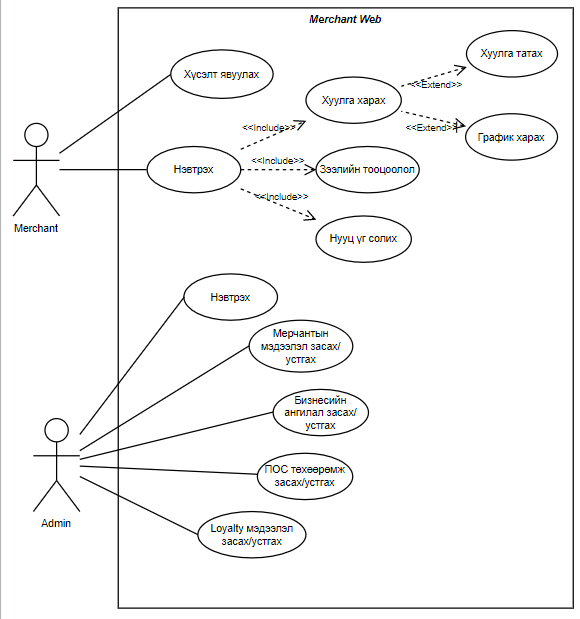
\includegraphics[width=13cm]{images/usecase.png}
	\caption{Use Case диаграм}
	\label{fig:form}
\end{figure}
